%%%%%%%%%%%%%%%%%%%% author.tex %%%%%%%%%%%%%%%%%%%%%%%%%%%%%%%%%%%
%
% sample root file for your "contribution" to a proceedings volume
%
% Use this file as a template for your own input.
%
%%%%%%%%%%%%%%%% Springer %%%%%%%%%%%%%%%%%%%%%%%%%%%%%%%%%%


\documentclass{svproc}
%
% RECOMMENDED %%%%%%%%%%%%%%%%%%%%%%%%%%%%%%%%%%%%%%%%%%%%%%%%%%%
%

% to typeset URLs, URIs, and DOIs
\usepackage{url}
\usepackage{graphicx}
\usepackage{amsmath}
\usepackage[utf8]{inputenc}
\usepackage{xcolor}
\def\UrlFont{\rmfamily}
\newcommand{\ottavia}[1]{\textcolor{purple}{#1}}
\newcommand{\livio}[1]{\textcolor{orange}{#1}}

\begin{document}
\mainmatter              % start of a contribution
%
\title{Nothing lasts forever -- only item administration: An Item Response Theory algorithm to shorten tests}
%
\titlerunning{IRT-based algorithms}  % abbreviated title (for running head)
%                                     also used for the TOC unless
%                                     \toctitle is used
%
\author{Ottavia M. Epifania\inst{1} and Livio Finos\inst{2}}
%
\authorrunning{Epifania \& Finos} % abbreviated author list (for running head)
%
%%%% list of authors for the TOC (use if author list has to be modified)
\tocauthor{Ottavia M. Epifania, Livio Finos}
%
\institute{Department of Psychology and Cognitive Science, University of Trento, IT\\
\email{ottavia.epifania@unitn.it}
\and
{\color{red}Department of Statistics, University of Padova, IT} \livio{devi vedere se è giusto} \\}

\maketitle              % typeset the title of the contribution

\begin{abstract}
\ottavia{da rivedere}
Although a larger number of test items improves measurement validity, the effect of respondents’ fatigue on the response quality should be acknowledged for developing reliable measurement tools.  This contribution presents an item response theory-based algorithm (denoted as Léon) able to shorten existing tests by concurrently accounting for the measurement precision of the abbreviated test and the tiredness of the respondents, which is here conceptualized as the probability of observing careless errors as the number of administered items increases. A simulation study compares the performance of Léon of approximating the measurement precision that would be obtained from the full-length test without the effect of the tiredness against that of another algorithm that does not account for the tiredness of the respondents. Although on average the two algorithms select the same number of items, Léon provides a better approximation to the measurement precision of the full-length test than the other algorithm.  
% We would like to encourage you to list your keywords within
% the abstract section using the \keywords{...} command.
\keywords{Item response theory, careless error, information functions, short test forms}
\end{abstract}
%
\section{Introduction}
%
As a general rule of thumb, the higher the number of items in a test, the better the measurement in terms of validity and reliability. However, there is a trade-off between the number of administered items and the response quality. As such, the trade-off between the number of administered items and the tiredness of the respondents \ottavia{(i.e., response fatigue)} should be kept in mind to obtain reliable and precise measurement tools. Item Response Theory (IRT, see, e.g., \cite{baker}) provides an ideal framework for shortening existing tests given the detailed information that they provide of the measurement precision of each item with respect to different levels of the latent trait (see e.g., \cite{pauci}). 
In this contribution, we present a new IRT-based algorithm for developing short test forms (STFs) from existing tests, denoted as Léon. This algorithm considers the response fatigue during the item selection process, such that it attempts at minimizing the number of selected items to maximize the measurement precision (as expressed by the test information function, TIF) of the STF.
%The ability of Léon of developing STFs able to approximate the TIF that would be obtained by administering all the items under the assumption that respondents would never get tired is investigated in a simulation study. 
%Specifically, Léon's ability is compared against that of another algorithm for developing STFs, which does not account for the tiredness of the respondents. 
The response fatigue has been here conceptualized as the careless error related to the item rank during the administration. 

\section{Item Response Theory and Information Functions}  

In IRT models for dichotomous responses (e.g., correct vs. incorrect), the probability of observing a correct response on item $i$ by person $p$ depends on both the charcteristics of the respondent (as described by their latent trait level, $\theta_p$) and on the characteristics of the item, which can be described by different parameters. IRT models differentiate according to the number of parameters used for describing the characteristics of the items. According to the 4-Parameter logistic model (4-PL, \cite{barton:4pl}), the probability of a correct response is: 

\begin{equation}\label{eq:4pl}
	P(x_{pi}= 1| \theta_p, b_i, a_i, c_i, d_i) = c_i + (d_i -c_i) + \dfrac{\exp[a_i(\theta_p - b_i)]}{1 + \exp[a_i(\theta_p - b_i)]},
\end{equation}
where $\theta_p$ is the latent trait level of person $p$, $b_i$ is the item location on the latent trait (i.e., difficulty parameter, the higher the value, the higher the difficulty of the item), and $a_i$ is the item ability to discriminate between respondents with different latent trait levels (i.e., discrimination parameter, the higher the value, the higher the discrimination ability of the item). Parameters $c_i$ and $d_i$ are the lower and upper asymptotes of the probability, which should naturally tend to 0 and 1 when $\theta \to - \infty$ and $\theta \to +\infty$, respectively. 
%However, there might instances where respondents with $\theta_p \to -\infty$ provide the correct response and respondents with $\theta_p \to + \infty$ do not provide the correct response.
%However, there might be instances where respondents with $\theta$ levels below the difficulty of the item, whom are hence expected not to respond correctly, might provide the correct response out of luck. 
The pseudoguessing parameter $c_i$ is the probability of observing a correct response on $i$ for $\theta \to - \infty$, such that the probability tends to $c_i$ instead of 0. 
%The same but inverse consideration applies when $\theta \to + \infty$. 
The $d_i$ parameter is the probability of observing a correct response on $i$ for $\theta \to + \infty$, such that this probability tends to $d_i$ instead of 1. The careless error probability is $1 - d_i$ (i.e., the probability of not endorsing the item given that the $\theta_p > b_i$).

%By constraining $\forall i \in B, \, d_i = 1$ (where $B$ is the set of items in a test) in equation \ref{eq:4pl}, the 3-Parameter logistic (3-PL, \cite{lord:3pl}) model is obtained. From the 3-PL model, the 2-Parameter logistic model (2-PL, \cite{birnbaum}) is obtained by constraining $\forall i \in B, \, c_i = 0$, and the 1-parameter logistic model (1-PL, equivalent to the Rasch model) is obtained by constraining $\forall i \in B, \, a_i = 1$. 

\ottavia{In this study, the response fatigue has been conceptualized as the careless error probability $1 - d_i$, which increases as the administration goes on. As $1 - d_i$ increases, the upper aymptote $d_i$ decreases.}
This probability is instrinsically related to the item rank in the test, hence the careless error parameter in Equation (\ref{eq:4pl}), which is usually a property of the item ($d_i$), becomes a property of the item rank $r = \{1, \ldots, R\}$ in the test, $d_r$, with the constraint $d_{r-1} > d_r$.
\normalcolor

\subsection{Information Functions}

The measurement precision of each item with respect to different levels of the latent trait is expressed by the \emph{item information functions} (IIFs). 
\color{blue}
Given that in this application the response fatigue has been conceptualized as the careless errors as the administration goes on, the typical formalization of the IIF for the 4-PL \cite{magis:iif} has been modified to account for the rank of presentation $r$ of item $i$, as follows:
\normalcolor


\begin{equation}\label{eq:iif}
	\text{IIF}_{i}(r) = \dfrac{a^2[P(\theta)-c_i]^2[d_r - P(\theta)]^2}{(d_{r}-c_i)^2 P(\theta)Q(\theta)}, 
\end{equation}
whereas in the typical formalization $d_r = d_i$.
%the $d$ parameter in Equation (\ref{eq:iif}) is a property related to its order of presentation in the test $r$, and it is hence denoted as $d_r$ with $r = \{1, \ldots, R\}$.
The $\text{IIF}_i$ is strongly influenced by the item location on the latent trait with respect to a specific $\theta_p$, its discriminativity, and its lucky guess and careless error. In absence of lucky guess and careless error, the IIF is maximum when  $\theta_p = b_i$, and it decreases as the distance between $b_i$ and $\theta_p$ increases. When the lucky guess and careless error are taken into account, the informativeness of the item decreases, the IIF is lower, and it maximum is shifted. 

The \emph{test information function} (TIF) is the sum of the IIFs, such that its shape (i.e., its informativeness with respect to different latent trait levels) and its height (i.e., the amount of information for different latent trait levels) depend on the items distribution along the latent trait. The more the items with high discrimination and low lucky guess and careless error parameters are spread throughout the latent trait, the more the test is informative of different regions. 


\section{Item Selection Algorithms}



The two algorithms (denoted as Frank and Léon) aim at reducing the distance between a target TIF (TIF-target, describes the desired measurement precision of the STFs) and a provisional TIF (pTIF) obtained from the items included in the STF. 
At each iteration, an item is included in the STF according to its ability of bridging the gap between the two TIFs. 
The algorithms stop when the distance between the TIF-target and the pTIF with the last considered item is equal to or greater than the distance between the TIF-target and the pTIF without the last considered items (i.e., termination criterion). 

In what follows, the TIF-target is represented by the TIF that would be obtained if respondents would never get tired during the administration of all the items in a test $B$. Therefore, the TIF-target is denoted as  $\text{TIF}_B$.

%The parameters of the items in $B$ are defined through an $I \times 4$ matrix, where $I$ is the total number of items in $B$ ($||B||$, where $||X||$ denotes the cardinality of set $X$) and the 4 columns contain the item parameters $b_i$, $a_i$, $c_i$, and $d_i$. 
Given that $B$ is the set of item without the effect of the tiredness, $d_i = 1$, $\forall i \in B$. To include the response fatigue, the vector of careless error parameters $d_r$ should be modified considering the item rank of presentation. In this application, $d_r$ is modified with an exponential function, $d_r = \exp(-\lambda r)$ (where $\lambda$ is the non-negative speed parameter determining the steepness of the function and $r$ is the rank of the $r$-th item in the administration). 
The items set with $d'$ is $B'$.

Since the TIF increases as the number of test items increases, the comparison between $\text{TIF}_B$ and the TIF of the STFs is based on the mean TIF (i.e., the TIF divided by the number of items). In what follows, the mean TIF  is simply referred to as $\text{TIF}_{Q_x}$, with $x \in \{B, B', \text{Frank}, \text{\text{Léon}}\}$ and $Q$ is the items set in the tests $B$ or $B'$ or the items subset in the STFs generated by the algorithms.

\subsection{Frank}

%\color{red}
%è qui che va detto che Frank calcola le iif di tutti gli item all'inizio e che poi vengono prese solo quelle degli item che sono disponibili in un dato momento, le IIF che sono in $A^k$
%\normalcolor


Frank selects the item whose IIF is best able to reduce the distance from the $\text{TIF}_B$ along the entire latent trait, as follows:


At $k = 0$: $\text{IIF}_i$, $\text{TIF}^0(\theta) = 0 \, \forall \theta$, $Q^0 = \emptyset$. For $k \geq 0$,

\begin{enumerate}
	\item  $A^k = B \setminus Q^k$ 
	\item $\forall i \in A^k$, $p\text{TIF}_{i}^k = \frac{\text{TIF}^k + \text{IIF}_{i}}{||Q^k||+1}$, with $c_i = 0$ and $d_i = 1$, $\forall i \in B$
	\item $i^* = \arg \min_{i \in A^k} (|\text{TIF}_B - \text{pTIF}_i^k|)$
	\item Termination criterion: $|\text{TIF}_B - \text{pTIF}_{i^*}^k| \geq |\text{TIF}_B - \text{TIF}^{k}|$: 
	\begin{itemize}
		\item FALSE:  $Q^{k+1} = Q^{k} \cup \{i^*\}$, $\text{TIF}^{k+1} = p\text{TIF}_{i^*}$, iterates 1-4 
		\item TRUE: Stop, %The item in $i^*$ does not contribute to reduce the distance from the TIF-target, hence: 
		$Q_{\text{Frank}} = Q^k$
		
	\end{itemize}
\end{enumerate}
At $k = 0$, the subset of items $Q^0$ is empty and the $\text{TIF}^0$ is 0 for all the $\theta$ levels. 
At each iteration $k$: (1.) a set of available items is generated as the items in the item bank that have not been included in the STF yet, $A^k = B \setminus Q^k$; (2.)
An average provisional TIF, $\text{pTIF}$, is computed by adding the IIF of each of the items in the set of the available items $A^k$, one at the time, to the TIF obtained from the items in $Q^k$ (The denominator is obtained by adding 1 to the cardinality of $Q^k$); (3.) Among all the items in $A^k$, the one that allows for minimizing the distance between $\text{pTIF}$ and $\text{TIF}_B$ is included in $i^*$; (4.) 
The termination criterion is tested. 
If the distance between the $\text{TIF}_B$ and the $\text{pTIF}_{i^*}$ is greater than or equal to the distance between the $\text{TIF}_B$ and the $\text{TIF}^k$ (i.e., the TIF obtained from the items in the subset $Q^k$, without item $i^*$) (TRUE), then the item $i^*$ does not contribute in the reduction of the distance from the $\text{TIF}_B$, the algorithm stops, and the final item selection is the one without the item in $i^*$, $Q_{frank} = Q^k$. Conversely (FALSE), the item in $i^*$ does contribute in the reduction of the distance from the $\text{TIF}_B$, hence it is included in the set of items and a new iteration starts, $Q^{k+1} = Q^k \cup \{i^*\}$.

\color{blue}
\subsection{Léon}
Differently from Frank, at step (2.) Léon computes the $\text{IIF}_i$ by considering the $d_r$ related to the number of items included in the STF up to that point.  
\normalcolor


\section{Simulation study}

\subsection{Simulation design}



The procedure is replicated 100 times. At each replication, a test $B$ of 50 items with difficulty ($b_i \sim \mathcal{U}(-3, 3)$) discrimination ($a_i \sim \mathcal{U}(.90, 2)$) parameters drawn from uniform distributions is generated. Lucky 
guess and careless error parameters are constant, $c_i = 0$ and $d_i = 1$, $\forall i \in B$.
The $\text{TIF}_B$ (i.e., the TIF-target) is obtained as the average TIF  from the items in $B$, and describes the measurement precision that would be obtained if respondents were administered with all the items without getting tired. 

At each replication, a new test, $B'$, is generated, where $b_i' = b_i$, $a_i' = a_i$, $c_i = 0$, $\forall i \in B'$, and $d_r = \exp(-\lambda r_i)$, with $\lambda = 0.01$ and $r = \{0, \ldots, ||B|| -1\}$.

At each replication, Frank and Léon generate a STF for approximating the $\text{TIF}_B$. An average TIF is computed considering the item in $B'$, denoted as $\text{TIF}_{B'}$.
Although Frank grounds the item selection on the set $B$, the final TIF is computed by considering the vector $d_r$ associated to the rank of the items in $Q_{\text{Frank}}$.
%La differenza è che Frank calcola tutte le iif degli tiem all'inizio, consdierando la careless error legata alla posizione dell'item così come viene generata inizialmente dalla funzione. 
%Léon invece calcola la iif ad ogni itereazione (per questo è più lento) mettendo dentro la careless error che è legata alla posizione dell'item. Nel senso, se Léon per ora ha selezionato 3 item e deve valutare se metterne un quarto, le iif degli item che sono rimasti verrà calcolata considerando la careless error in $B'$ dell'item somministrato per quarto.
\normalcolor


\subsection{Comparison}

The average distance from $\text{TIF}_B$ of the STFs generated by Frank and Léon at each iteration, as well as of the test obtained from $B'$ has been considered as a criterion for evaluating the ability of Léon of generating informative STFs while accounting for the tiredness of the respondents, $\Delta_x = |\text{TIF}_B - \text{TIF}_{Q_x}|$, with $x \in \{B', \text{Frank}, \text{Léon}\}$.  Trivially, when the $\text{TIF}_{B'}$ is considered, $Q = B'$.

To better understand whether acknowledging the tiredness of the respondents influences the number of items included in $Q$, the cardinalities of the STFs generated by Frank and Léon, $||Q_{\text{Frank}}||$ and $||Q_{\text{Léon}}||$, respectively, have been compared. 

%Moreover, the TIF of the items in $B'$ has been computed as well and compared against those of the STFs resulting from the application of Frank and Léon. 
%The rationale is as follows. The more the item in a test, the higher the information for different regions of the latent trait. 
%However, administering too many items might be an highly demanding task, such that the respondent might get tired and their response accuracy might decrease during the administration, such that the last administered items might include error variance not related to the construct under investigation. 
%In this light, it should be more convenient to administer less but highly informative items, able to approximate a specific TIF target, than to administer the entire test to obtain precise measurements of the latent trait.
  

\section{Results}

%Table \ref{tab:summary} illustrates the mean distance of $\text{TIF}_x$, $x \in \{B', Q_{\text{Frank}}, Q_{\text{Léon}}\}$ from $TIF^*$, computed across the 100 replications. 
%
%\begin{table}
%	\centering
%	\caption{\label{tab:summary} Average distance from the $\text{TIF}^*$.}
%	\begin{tabular}{l ccc}
%		\hline
%	Procedure	&	M			&	Min	&	Max	\\\hline
%	All items	& $	0.07\pm	0.03$ &	$< 0.005$	&	0.13	\\
%	Frank	& $	0.03	\pm	0.03	$ &	$<0.001$	&	0.14	\\
%	Léon	& $	0.03	\pm	0.02	$ &	$<0.001$	&	0.10	\\
%	\hline	
%	\end{tabular}
%	\flushleft \emph{Note:} All items: TIF obtained considering all the items in $B'$; Frank: STFs obtained without considering the tiredness of the respondents in the item selection; Léon: STFs obtained by considering the tiredness of the respondents in the item selection.
%\end{table}

On average, Léon and Frank included the same number of items in the STF, $M_{\text{Léon}} = 6.75 \pm 3.06$, $M_{\text{Frank}} = 6.31 \pm 2.40$, $t = 1.13$, $df = 187.59$, $p = .26$, suggesting that accounting for the tiredness of the respondents does not influence the number of items included in the STF.
%\color{red}
%Given that leon account for the tiredness of the respondents during the item selection, it also considers the measurement precision of the STF given that the respondents do get tired during the administration, while Frank does not. As such, while preventing the over inclusion of items in the STF, Léon is also able to account for the measurement precision, in the attempt of balancing the number of items with the measurement precision.
%\normalcolor

Figure \ref{fig:points-alogirthms} illustrates the distributions of the distances from $\text{TIF}_B$ ($y$-axis) of $Q_x$ ($x$-axis).

\begin{figure}[!h]
	\centering
	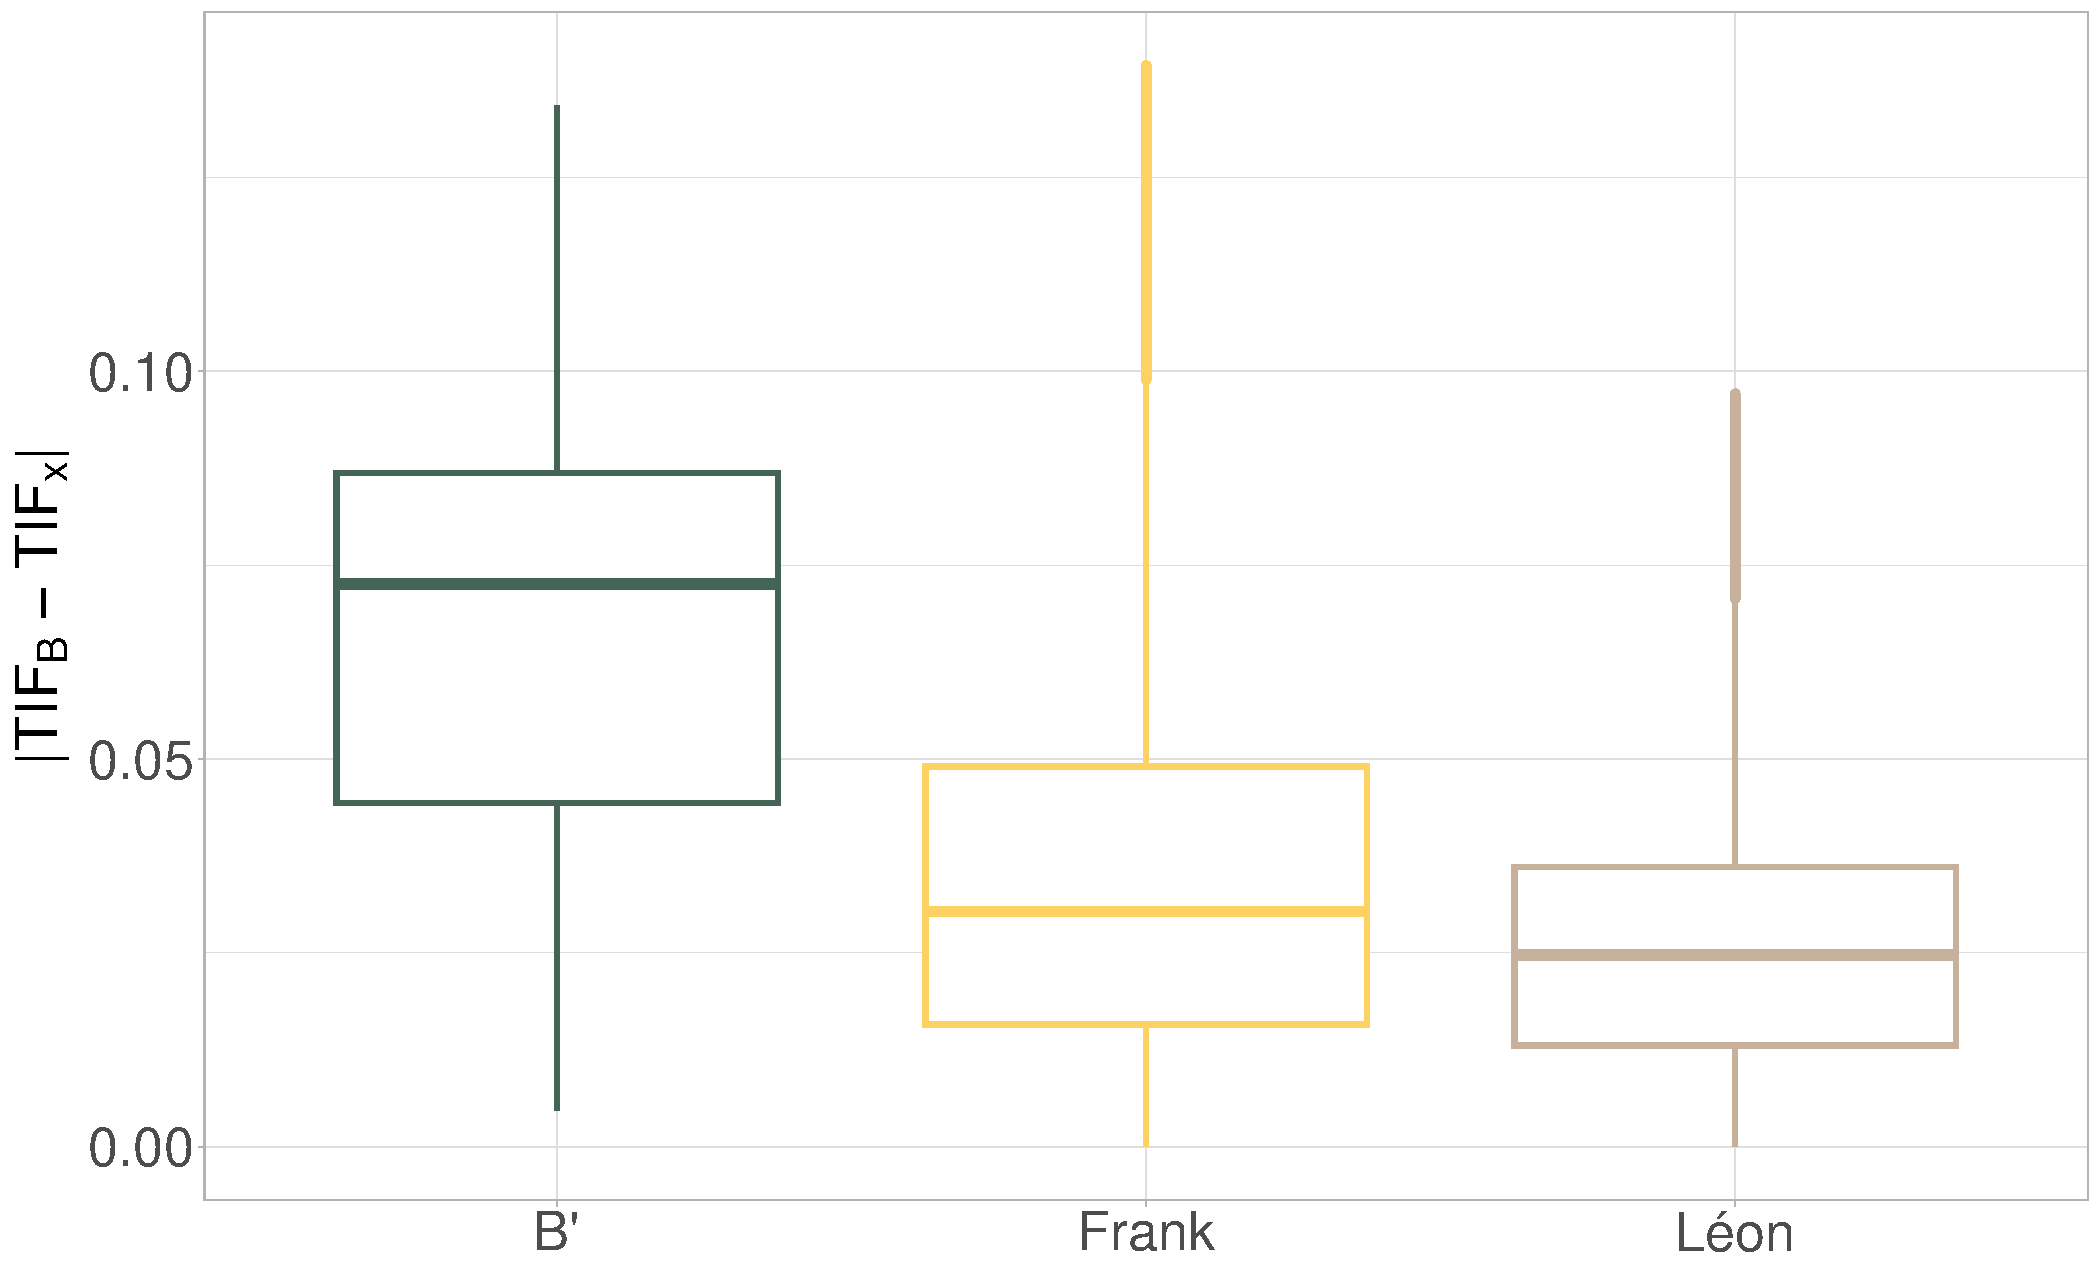
\includegraphics[width=\linewidth]{img/box-plot-alogirthms}
	\caption{Distance from $\text{TIF}_{B}$ of $\text{TIF}_{B'}$, $\text{TIF}_{\text{Frank}}$, and $\text{TIF}_{\text{Léon}}$  across the 100 replications.} 
	\label{fig:points-alogirthms}
\end{figure}

Overall, $\text{TIF}_{B'}$s are the most distant from $\text{TIF}_B$, while $\text{TIF}_{\text{Léon}}$s are the closest ones. Frank falls in between the two, also presenting the least consistent performance across the replications. 

\section{Final Remarks}

This manuscript presented an IRT-based algorithm, denoted as Léon, for the generation of  STFs. 
Léon grounds the item selection by concurrently considering the number of items included in the STF and the measurement precision with respect to an ideal target where all the items are administered in absence of careless error (i.e., TIF-target). The ability of Léon of approximating the TIF-target has been compared against that of another algorithm (Frank) not accounting for the response fatigue during item selection and with the measurement precision obtained from the administration of the entire test, including the careless mistakes due to the response fatigue.
 

Generally, the results suggest that the administration of fewer items provide better measurement tools than administering the entire test, especially if the selection process accounts for the effect of the response fatigue.

Although the results are promising, several limitations must be acknowledged. Firstly, while this study primarily focuses on approximating ideal measurement precision as expressed by the TIF-target, no investigations on the precision with which the latent trait is estimated with the STFs are presented. Future studies should further investigate this issue to understand whether administering less items brings actual benefits in the estimation of the latent trait.
Secondly, the operalization of the tiredness of the response fatigue as an increase of the probability of committing careless error as the administration goes on is an arbitrary choice, and other possibilities should be investigated.




% ---- Bibliography ----
%
\begin{thebibliography}{6}
%

\bibitem {baker}
 Baker, F. B., Kim, S.-H. (2017). The basics of Item Response Theory using R. Springer.

\bibitem {barton:4pl}
Barton, M. A., Lord, F. M. (1981). An upper asymptote for the three-parameter logistic item-response
model. Princeton, NJ: Educational Testing Service.


\bibitem{pauci}

Epifania, O.M., Anselmi, P., Robusto, E. (2022). Pauci sed boni: An Item Response Theory Approach for Shortening Tests. In: Wiberg, M.,et al. (eds) \textit{Quantitative Psychology.} IMPS 2022. Springer Proceedings in Mathematics \& Statistics, vol 422. Springer, Cham. \url{https://doi.org/10.1007/978-3-031-27781-87}

%\bibitem {birnbaum}
%Birnbaum, A. (1968). Some latent trait models and their use in inferring an examinee’s ability. In F. M.
%Lord, M. R. Novick (Eds.), Statistical theories of mental test scores (pp. 397-479). Reading, MA:
%Addison-Wesley

%\bibitem {lord:3pl}
%Lord, F. M. (1980). Applications of item response theory to practical testing problems. Hillsdale, NJ:
%Lawrence Erlbaum

\bibitem {magis:iif}
Magis, D. (2013). A note on the item information function of the four-parameter logistic model. Applied Psychological Measurement, 37(4), 304-315.


%\bibitem {rsoft}
%R Development Core Team. (2012). R: A language and environment for statistical computing [Computer
%software]. Vienna, Austria: R Foundation for Statistical Computing.




\end{thebibliography}
\end{document}
